% Options for packages loaded elsewhere
\PassOptionsToPackage{unicode}{hyperref}
\PassOptionsToPackage{hyphens}{url}
%
\documentclass[
]{article}
\usepackage{lmodern}
\usepackage{amssymb,amsmath}
\usepackage{ifxetex,ifluatex}
\ifnum 0\ifxetex 1\fi\ifluatex 1\fi=0 % if pdftex
  \usepackage[T1]{fontenc}
  \usepackage[utf8]{inputenc}
  \usepackage{textcomp} % provide euro and other symbols
\else % if luatex or xetex
  \usepackage{unicode-math}
  \defaultfontfeatures{Scale=MatchLowercase}
  \defaultfontfeatures[\rmfamily]{Ligatures=TeX,Scale=1}
\fi
% Use upquote if available, for straight quotes in verbatim environments
\IfFileExists{upquote.sty}{\usepackage{upquote}}{}
\IfFileExists{microtype.sty}{% use microtype if available
  \usepackage[]{microtype}
  \UseMicrotypeSet[protrusion]{basicmath} % disable protrusion for tt fonts
}{}
\makeatletter
\@ifundefined{KOMAClassName}{% if non-KOMA class
  \IfFileExists{parskip.sty}{%
    \usepackage{parskip}
  }{% else
    \setlength{\parindent}{0pt}
    \setlength{\parskip}{6pt plus 2pt minus 1pt}}
}{% if KOMA class
  \KOMAoptions{parskip=half}}
\makeatother
\usepackage{xcolor}
\IfFileExists{xurl.sty}{\usepackage{xurl}}{} % add URL line breaks if available
\IfFileExists{bookmark.sty}{\usepackage{bookmark}}{\usepackage{hyperref}}
\hypersetup{
  pdftitle={Practical 05 SG: Population substructure},
  pdfauthor={Lovro Katalinic and Ivan Almer},
  hidelinks,
  pdfcreator={LaTeX via pandoc}}
\urlstyle{same} % disable monospaced font for URLs
\usepackage[margin=1in]{geometry}
\usepackage{color}
\usepackage{fancyvrb}
\newcommand{\VerbBar}{|}
\newcommand{\VERB}{\Verb[commandchars=\\\{\}]}
\DefineVerbatimEnvironment{Highlighting}{Verbatim}{commandchars=\\\{\}}
% Add ',fontsize=\small' for more characters per line
\usepackage{framed}
\definecolor{shadecolor}{RGB}{248,248,248}
\newenvironment{Shaded}{\begin{snugshade}}{\end{snugshade}}
\newcommand{\AlertTok}[1]{\textcolor[rgb]{0.94,0.16,0.16}{#1}}
\newcommand{\AnnotationTok}[1]{\textcolor[rgb]{0.56,0.35,0.01}{\textbf{\textit{#1}}}}
\newcommand{\AttributeTok}[1]{\textcolor[rgb]{0.77,0.63,0.00}{#1}}
\newcommand{\BaseNTok}[1]{\textcolor[rgb]{0.00,0.00,0.81}{#1}}
\newcommand{\BuiltInTok}[1]{#1}
\newcommand{\CharTok}[1]{\textcolor[rgb]{0.31,0.60,0.02}{#1}}
\newcommand{\CommentTok}[1]{\textcolor[rgb]{0.56,0.35,0.01}{\textit{#1}}}
\newcommand{\CommentVarTok}[1]{\textcolor[rgb]{0.56,0.35,0.01}{\textbf{\textit{#1}}}}
\newcommand{\ConstantTok}[1]{\textcolor[rgb]{0.00,0.00,0.00}{#1}}
\newcommand{\ControlFlowTok}[1]{\textcolor[rgb]{0.13,0.29,0.53}{\textbf{#1}}}
\newcommand{\DataTypeTok}[1]{\textcolor[rgb]{0.13,0.29,0.53}{#1}}
\newcommand{\DecValTok}[1]{\textcolor[rgb]{0.00,0.00,0.81}{#1}}
\newcommand{\DocumentationTok}[1]{\textcolor[rgb]{0.56,0.35,0.01}{\textbf{\textit{#1}}}}
\newcommand{\ErrorTok}[1]{\textcolor[rgb]{0.64,0.00,0.00}{\textbf{#1}}}
\newcommand{\ExtensionTok}[1]{#1}
\newcommand{\FloatTok}[1]{\textcolor[rgb]{0.00,0.00,0.81}{#1}}
\newcommand{\FunctionTok}[1]{\textcolor[rgb]{0.00,0.00,0.00}{#1}}
\newcommand{\ImportTok}[1]{#1}
\newcommand{\InformationTok}[1]{\textcolor[rgb]{0.56,0.35,0.01}{\textbf{\textit{#1}}}}
\newcommand{\KeywordTok}[1]{\textcolor[rgb]{0.13,0.29,0.53}{\textbf{#1}}}
\newcommand{\NormalTok}[1]{#1}
\newcommand{\OperatorTok}[1]{\textcolor[rgb]{0.81,0.36,0.00}{\textbf{#1}}}
\newcommand{\OtherTok}[1]{\textcolor[rgb]{0.56,0.35,0.01}{#1}}
\newcommand{\PreprocessorTok}[1]{\textcolor[rgb]{0.56,0.35,0.01}{\textit{#1}}}
\newcommand{\RegionMarkerTok}[1]{#1}
\newcommand{\SpecialCharTok}[1]{\textcolor[rgb]{0.00,0.00,0.00}{#1}}
\newcommand{\SpecialStringTok}[1]{\textcolor[rgb]{0.31,0.60,0.02}{#1}}
\newcommand{\StringTok}[1]{\textcolor[rgb]{0.31,0.60,0.02}{#1}}
\newcommand{\VariableTok}[1]{\textcolor[rgb]{0.00,0.00,0.00}{#1}}
\newcommand{\VerbatimStringTok}[1]{\textcolor[rgb]{0.31,0.60,0.02}{#1}}
\newcommand{\WarningTok}[1]{\textcolor[rgb]{0.56,0.35,0.01}{\textbf{\textit{#1}}}}
\usepackage{graphicx,grffile}
\makeatletter
\def\maxwidth{\ifdim\Gin@nat@width>\linewidth\linewidth\else\Gin@nat@width\fi}
\def\maxheight{\ifdim\Gin@nat@height>\textheight\textheight\else\Gin@nat@height\fi}
\makeatother
% Scale images if necessary, so that they will not overflow the page
% margins by default, and it is still possible to overwrite the defaults
% using explicit options in \includegraphics[width, height, ...]{}
\setkeys{Gin}{width=\maxwidth,height=\maxheight,keepaspectratio}
% Set default figure placement to htbp
\makeatletter
\def\fps@figure{htbp}
\makeatother
\setlength{\emergencystretch}{3em} % prevent overfull lines
\providecommand{\tightlist}{%
  \setlength{\itemsep}{0pt}\setlength{\parskip}{0pt}}
\setcounter{secnumdepth}{-\maxdimen} % remove section numbering

\title{Practical 05 SG: Population substructure}
\author{Lovro Katalinic and Ivan Almer}
\date{Hand-in: 21/12/2020}

\begin{document}
\maketitle

Resolve the following exercise in groups of two students. Perform the
computations and make the graphics that are asked for in the practical
below. Take care to give each graph a title, and clearly label \(x\) and
\(y\) axes, and to answer all questions asked. You can write your
solution in a word or Latex document and generate a pdf file with your
solution. Alternatively, you may generate a solution pdf file with
Markdown. You can use R packages \textbf{genetics}, \textbf{MASS},
\textbf{data.table} and others for the computations. Take care to number
your answer exactly as in this exercise. Upload your solution in
\textbf{pdf format} to the web page of the course at raco.fib.upc.edu no
later than the hand-in date.

\begin{verbatim}
## Loading required package: combinat
\end{verbatim}

\begin{verbatim}
## 
## Attaching package: 'combinat'
\end{verbatim}

\begin{verbatim}
## The following object is masked from 'package:utils':
## 
##     combn
\end{verbatim}

\begin{verbatim}
## Loading required package: gdata
\end{verbatim}

\begin{verbatim}
## gdata: read.xls support for 'XLS' (Excel 97-2004) files ENABLED.
\end{verbatim}

\begin{verbatim}
## 
\end{verbatim}

\begin{verbatim}
## gdata: read.xls support for 'XLSX' (Excel 2007+) files ENABLED.
\end{verbatim}

\begin{verbatim}
## 
## Attaching package: 'gdata'
\end{verbatim}

\begin{verbatim}
## The following object is masked from 'package:stats':
## 
##     nobs
\end{verbatim}

\begin{verbatim}
## The following object is masked from 'package:utils':
## 
##     object.size
\end{verbatim}

\begin{verbatim}
## The following object is masked from 'package:base':
## 
##     startsWith
\end{verbatim}

\begin{verbatim}
## Loading required package: gtools
\end{verbatim}

\begin{verbatim}
## Loading required package: MASS
\end{verbatim}

\begin{verbatim}
## Loading required package: mvtnorm
\end{verbatim}

\begin{verbatim}
## 
\end{verbatim}

\begin{verbatim}
## NOTE: THIS PACKAGE IS NOW OBSOLETE.
\end{verbatim}

\begin{verbatim}
## 
\end{verbatim}

\begin{verbatim}
##   The R-Genetics project has developed an set of enhanced genetics
\end{verbatim}

\begin{verbatim}
##   packages to replace 'genetics'. Please visit the project homepage
\end{verbatim}

\begin{verbatim}
##   at http://rgenetics.org for informtion.
\end{verbatim}

\begin{verbatim}
## 
\end{verbatim}

\begin{verbatim}
## 
## Attaching package: 'genetics'
\end{verbatim}

\begin{verbatim}
## The following objects are masked from 'package:base':
## 
##     %in%, as.factor, order
\end{verbatim}

\begin{verbatim}
## 
## Attaching package: 'data.table'
\end{verbatim}

\begin{verbatim}
## The following objects are masked from 'package:gdata':
## 
##     first, last
\end{verbatim}

\begin{enumerate}
\def\labelenumi{\arabic{enumi}.}
\tightlist
\item
  The file
  \href{http://www-eio.upc.es/~jan/data/bsg/Chr21.dat}{Chr21.dat}
  contains genotype information of a set of individuals of unknown
  background. Load this data into the R environment with the
  \emph{fread} instruction. The first six columns of the data matrix
  contain identifiers, sex and phenotype and are not needed. The
  remaining columns contain the allele counts (0, 1 or 2) for over
  138.000 SNPs for one of the alleles of each SNP.
\end{enumerate}

\begin{Shaded}
\begin{Highlighting}[]
\NormalTok{dataset =}\StringTok{ }\KeywordTok{fread}\NormalTok{(}\StringTok{'Chr21.dat'}\NormalTok{, }\DataTypeTok{data.table =} \OtherTok{FALSE}\NormalTok{)}
\NormalTok{dataset =}\StringTok{ }\NormalTok{dataset[,}\DecValTok{7}\OperatorTok{:}\KeywordTok{ncol}\NormalTok{(dataset)]}
\end{Highlighting}
\end{Shaded}

\begin{enumerate}
\def\labelenumi{\arabic{enumi}.}
\setcounter{enumi}{1}
\tightlist
\item
  (1p) Compute the \emph{Manhattan distance} matrix between the
  individuals (this may take a few minutes) using R function
  \texttt{dist}. Include a submatrix of dimension 5 by 5 with the
  distances between the first 5 individuals in your report.
\end{enumerate}

\begin{Shaded}
\begin{Highlighting}[]
\NormalTok{dists.all =}\StringTok{ }\KeywordTok{as.matrix}\NormalTok{(}\KeywordTok{dist}\NormalTok{(dataset, }\DataTypeTok{method =} \StringTok{'manhattan'}\NormalTok{))}

\NormalTok{dists =}\StringTok{ }\KeywordTok{dist}\NormalTok{(dataset[}\DecValTok{1}\OperatorTok{:}\DecValTok{5}\NormalTok{,], }\DataTypeTok{method =} \StringTok{'manhattan'}\NormalTok{)}
\NormalTok{d =}\StringTok{ }\KeywordTok{matrix}\NormalTok{(}\DataTypeTok{nrow =} \DecValTok{5}\NormalTok{, }\DataTypeTok{ncol =} \DecValTok{5}\NormalTok{)}

\NormalTok{dists.arr =}\StringTok{ }\KeywordTok{c}\NormalTok{(dists)}
\NormalTok{count =}\StringTok{ }\DecValTok{1}

\ControlFlowTok{for}\NormalTok{(i }\ControlFlowTok{in} \DecValTok{1}\OperatorTok{:}\NormalTok{(}\KeywordTok{nrow}\NormalTok{(d) }\OperatorTok{-}\StringTok{ }\DecValTok{1}\NormalTok{)) \{}
  \ControlFlowTok{for}\NormalTok{(j }\ControlFlowTok{in}\NormalTok{ (i}\OperatorTok{+}\DecValTok{1}\NormalTok{)}\OperatorTok{:}\NormalTok{(}\KeywordTok{ncol}\NormalTok{(d))) \{}
    \CommentTok{#print(dists.arr[count])}
\NormalTok{    d[i,j] =}\StringTok{ }\NormalTok{dists.arr[count]}
\NormalTok{    d[j,i] =}\StringTok{ }\NormalTok{dists.arr[count]}
\NormalTok{    count =}\StringTok{ }\NormalTok{count }\OperatorTok{+}\StringTok{ }\DecValTok{1}
\NormalTok{  \}}
\NormalTok{\}}

\NormalTok{d[}\KeywordTok{is.na}\NormalTok{(d)] =}\StringTok{ }\FloatTok{0.0}
\NormalTok{d}
\end{Highlighting}
\end{Shaded}

\begin{verbatim}
##       [,1]  [,2]  [,3]  [,4]  [,5]
## [1,]     0 53495 55007 58174 53794
## [2,] 53495     0 55372 55995 55699
## [3,] 55007 55372     0 54815 55683
## [4,] 58174 55995 54815     0 59046
## [5,] 53794 55699 55683 59046     0
\end{verbatim}

\begin{enumerate}
\def\labelenumi{\arabic{enumi}.}
\setcounter{enumi}{2}
\tightlist
\item
  (1p) The Manhattan distance (also known as the \emph{taxicab metric})
  is identical to the Minkowsky distance with parameter \(\lambda = 1\).
  How does the Manhattan distance relate to the allele sharing distance,
  where the latter is calculated as two minus the number of shared
  alleles?
\end{enumerate}

Manhattan distance is actually the same as Allele sharing distance since
distance. Let's see and example: manhattan distance for one variant with
values \(0\) and \(2\) (let's say AA and BB) is \textbar0-2\textbar{} =
2 and the allele sharing distance is 2-(number of shared alleles) = 2 -
0 = 2. This can be shown for every combination of variants. Obviously if
we scale the Allele sharing distance with number of variants we obtain
the results which is smaller than Manhattan distance but they are
proportional with the coefficiet \(1/K\) where \(K\) is the number of
variants.

\begin{enumerate}
\def\labelenumi{\arabic{enumi}.}
\setcounter{enumi}{3}
\tightlist
\item
  (2p) Apply metric multidimensional scaling using the Manhattan
  distance matrix to obtain a map of the individuals, and include your
  map in your report. Do you think the data come from one homogeneous
  human population? If not, how many subpopulations do you think the
  data might come from, and how many individuals pertain to each
  suppopulation?
\end{enumerate}

\begin{Shaded}
\begin{Highlighting}[]
\NormalTok{mds.out <-}\StringTok{ }\KeywordTok{cmdscale}\NormalTok{(dists.all,}\DataTypeTok{k=}\DecValTok{2}\NormalTok{,}\DataTypeTok{eig=}\OtherTok{TRUE}\NormalTok{)}

\NormalTok{X <-}\StringTok{ }\NormalTok{mds.out}\OperatorTok{$}\NormalTok{points[,}\DecValTok{1}\OperatorTok{:}\DecValTok{2}\NormalTok{]}
\KeywordTok{plot}\NormalTok{(X[,}\DecValTok{1}\NormalTok{],X[,}\DecValTok{2}\NormalTok{],}\DataTypeTok{asp=}\DecValTok{1}\NormalTok{,}\DataTypeTok{xlab=}\StringTok{"First principal axis"}\NormalTok{, }\DataTypeTok{ylab=}\StringTok{"Second principal axis"}\NormalTok{)}
\end{Highlighting}
\end{Shaded}

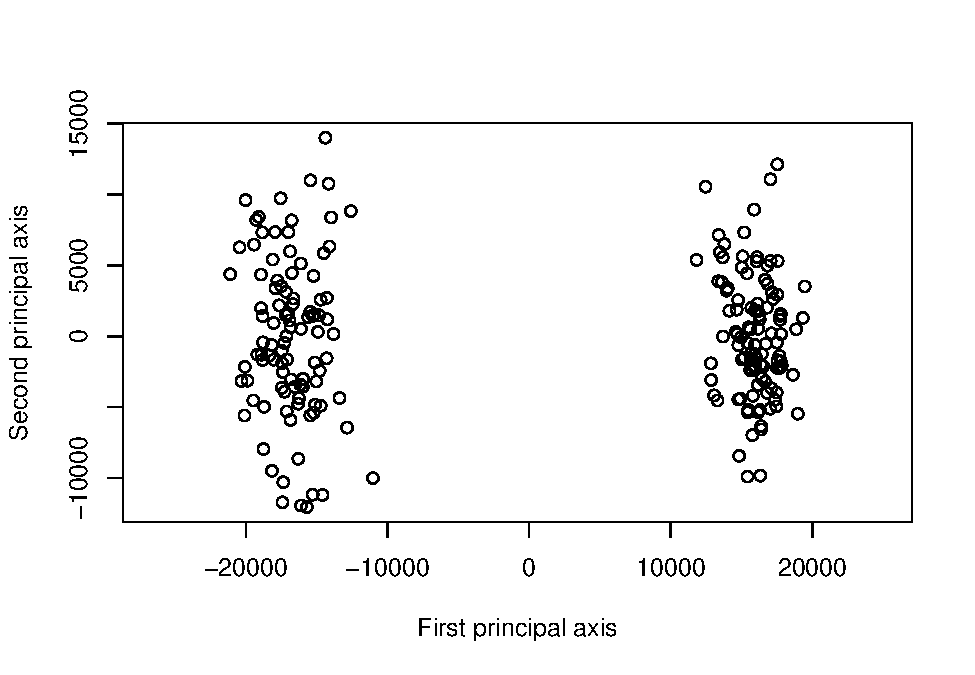
\includegraphics{P052020_Substructure_files/figure-latex/4th-1.pdf}

\begin{Shaded}
\begin{Highlighting}[]
\NormalTok{X.mds =}\StringTok{ }\NormalTok{X}

\NormalTok{left.pop =}\StringTok{ }\KeywordTok{sum}\NormalTok{(X[,}\DecValTok{1}\NormalTok{] }\OperatorTok{<}\StringTok{ }\DecValTok{0}\NormalTok{)}
\NormalTok{left.pop}
\end{Highlighting}
\end{Shaded}

\begin{verbatim}
## [1] 99
\end{verbatim}

\begin{Shaded}
\begin{Highlighting}[]
\NormalTok{right.pop =}\StringTok{ }\KeywordTok{sum}\NormalTok{(X[,}\DecValTok{1}\NormalTok{] }\OperatorTok{>}\StringTok{ }\DecValTok{0}\NormalTok{)}
\NormalTok{right.pop}
\end{Highlighting}
\end{Shaded}

\begin{verbatim}
## [1] 104
\end{verbatim}

There seem to exist 2 subpopulations i the shown population. In the
``left'' population there are 99 units and in the ``right'' population
there are 104 units.

\begin{enumerate}
\def\labelenumi{\arabic{enumi}.}
\setcounter{enumi}{4}
\tightlist
\item
  (1p) Report the first 10 eigenvalues of the solution.
\end{enumerate}

\begin{Shaded}
\begin{Highlighting}[]
\NormalTok{mds.out}\OperatorTok{$}\NormalTok{eig[}\DecValTok{1}\OperatorTok{:}\DecValTok{10}\NormalTok{]}
\end{Highlighting}
\end{Shaded}

\begin{verbatim}
##  [1] 54920034481  5138177890  4707357775  4643815383  4475557521  4247865984
##  [7]  4207565510  4078798696  3913698113  3895665124
\end{verbatim}

\begin{enumerate}
\def\labelenumi{\arabic{enumi}.}
\setcounter{enumi}{5}
\tightlist
\item
  (1p) Does a perfect representation of this \(n \times n\) distance
  matrix exist, in \(n\) or fewer dimensions? Why so or not?
\end{enumerate}

A perfect representation of the distance matrix does not exist because
by reducing dimensions we take away the degrees of freedom which enable
the original distance matrix to be such as it is.

\begin{enumerate}
\def\labelenumi{\arabic{enumi}.}
\setcounter{enumi}{6}
\tightlist
\item
  (1p) What is the goodness-of-fit of a two-dimensional approximation to
  your distance matrix? Explain which criterium you have used.
\end{enumerate}

/

\begin{enumerate}
\def\labelenumi{\arabic{enumi}.}
\setcounter{enumi}{7}
\tightlist
\item
  (2p) Make a plot of the estimated distances (according to your map of
  individuals) versus the observed distances. What do you observe?
  Regress estimated distances on observed distances and report the
  coefficient of determination of the regression.
\end{enumerate}

\begin{Shaded}
\begin{Highlighting}[]
\NormalTok{approx.dist =}\StringTok{ }\KeywordTok{as.matrix}\NormalTok{(}\KeywordTok{dist}\NormalTok{(X, }\DataTypeTok{method =} \StringTok{'manhattan'}\NormalTok{))}

\NormalTok{Dobs.vec <-}\StringTok{ }\NormalTok{dists.all[}\KeywordTok{lower.tri}\NormalTok{(dists.all)]}
\NormalTok{Dest.vec <-}\StringTok{ }\NormalTok{approx.dist[}\KeywordTok{lower.tri}\NormalTok{(approx.dist)]}

\KeywordTok{plot}\NormalTok{(Dobs.vec,Dest.vec,}\DataTypeTok{xlab=}\StringTok{"Observed"}\NormalTok{,}\DataTypeTok{ylab=}\StringTok{"Fitted"}\NormalTok{)}
\NormalTok{model =}\StringTok{ }\KeywordTok{lm}\NormalTok{(Dest.vec }\OperatorTok{~}\StringTok{ }\NormalTok{Dobs.vec)}
\KeywordTok{abline}\NormalTok{(model)}
\end{Highlighting}
\end{Shaded}

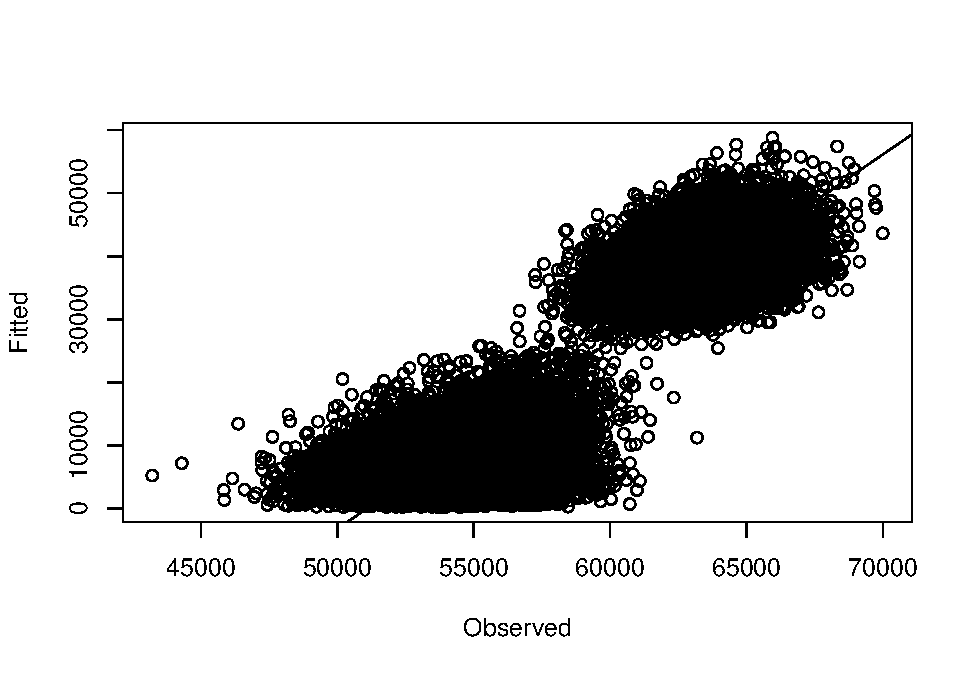
\includegraphics{P052020_Substructure_files/figure-latex/8th-1.pdf}

\begin{Shaded}
\begin{Highlighting}[]
\NormalTok{r2 =}\StringTok{ }\KeywordTok{summary}\NormalTok{(model)}\OperatorTok{$}\NormalTok{r.squared}
\NormalTok{r2}
\end{Highlighting}
\end{Shaded}

\begin{verbatim}
## [1] 0.8240959
\end{verbatim}

\begin{enumerate}
\def\labelenumi{\arabic{enumi}.}
\setcounter{enumi}{8}
\tightlist
\item
  (1p) We now try non-metric multidimensional scaling using the
  \texttt{isoMDs} instruction. We use a random initial configuration.
  For the sake of reproducibility, make this random initial
  configuration with the instructions:

  \begin{verbatim}
  set.seed(12345)
  init <- scale(matrix(runif(2*n),ncol=2),scale=FALSE)
  \end{verbatim}

  where \(n\) represents the sample size. Make a plot of the
  two-dimensional solution. Do the results support that the data come
  from one homogeneous population? Try some additional runs of
  \texttt{isoMDS} with different initial configurations, or eventually
  using the classical metric solution as the initial solution. What do
  you observe?
\end{enumerate}

\begin{Shaded}
\begin{Highlighting}[]
\NormalTok{n =}\StringTok{ }\KeywordTok{nrow}\NormalTok{(dataset)}
\KeywordTok{set.seed}\NormalTok{(}\DecValTok{12345}\NormalTok{)}

\NormalTok{init <-}\StringTok{ }\KeywordTok{scale}\NormalTok{(}\KeywordTok{matrix}\NormalTok{(}\KeywordTok{runif}\NormalTok{(}\DecValTok{2}\OperatorTok{*}\NormalTok{n),}\DataTypeTok{ncol=}\DecValTok{2}\NormalTok{),}\DataTypeTok{scale=}\OtherTok{FALSE}\NormalTok{)}
\NormalTok{nmds.out <-}\StringTok{ }\KeywordTok{isoMDS}\NormalTok{(dists.all,}\DataTypeTok{k=}\DecValTok{2}\NormalTok{,}\DataTypeTok{y=}\NormalTok{init, }\DataTypeTok{trace =} \OtherTok{FALSE}\NormalTok{)}
\NormalTok{X =}\StringTok{ }\NormalTok{nmds.out}\OperatorTok{$}\NormalTok{points}
\KeywordTok{plot}\NormalTok{(X[,}\DecValTok{1}\NormalTok{],X[,}\DecValTok{2}\NormalTok{],}\DataTypeTok{asp=}\DecValTok{1}\NormalTok{,}\DataTypeTok{xlab=}\StringTok{"First principal axis"}\NormalTok{, }\DataTypeTok{ylab=}\StringTok{"Second principal axis"}\NormalTok{)}
\end{Highlighting}
\end{Shaded}

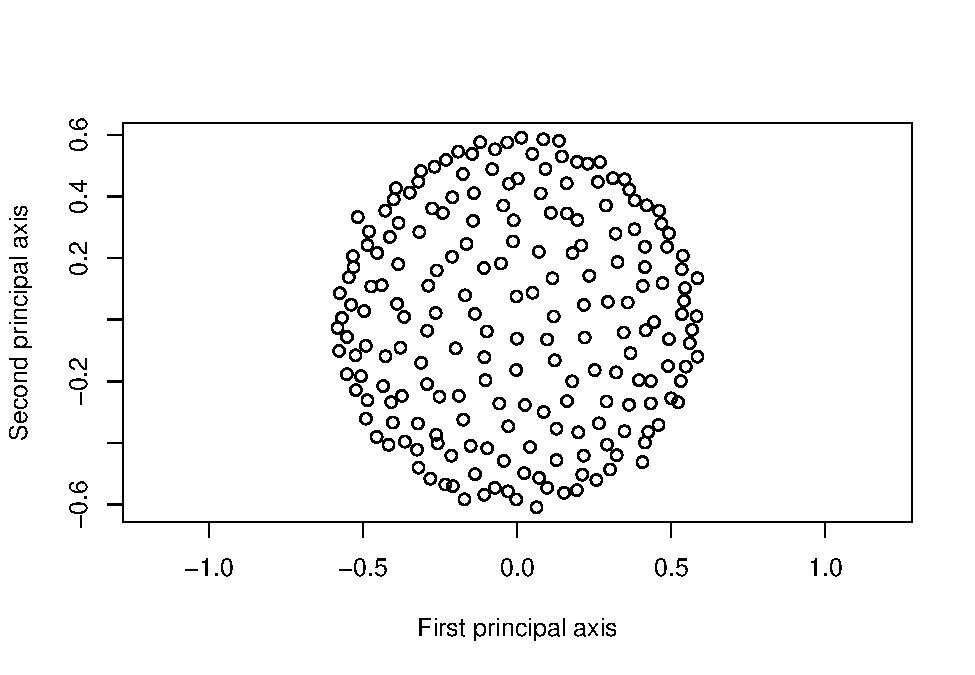
\includegraphics{P052020_Substructure_files/figure-latex/9th-1.pdf}

\begin{Shaded}
\begin{Highlighting}[]
\NormalTok{init <-}\StringTok{ }\KeywordTok{scale}\NormalTok{(}\KeywordTok{matrix}\NormalTok{(}\KeywordTok{runif}\NormalTok{(}\DecValTok{2}\OperatorTok{*}\NormalTok{n),}\DataTypeTok{ncol=}\DecValTok{2}\NormalTok{),}\DataTypeTok{scale=}\OtherTok{FALSE}\NormalTok{)}
\NormalTok{nmds.out <-}\StringTok{ }\KeywordTok{isoMDS}\NormalTok{(dists.all,}\DataTypeTok{k=}\DecValTok{2}\NormalTok{,}\DataTypeTok{y=}\NormalTok{init, }\DataTypeTok{trace =} \OtherTok{FALSE}\NormalTok{)}
\NormalTok{X =}\StringTok{ }\NormalTok{nmds.out}\OperatorTok{$}\NormalTok{points}
\KeywordTok{plot}\NormalTok{(X[,}\DecValTok{1}\NormalTok{],X[,}\DecValTok{2}\NormalTok{],}\DataTypeTok{asp=}\DecValTok{1}\NormalTok{,}\DataTypeTok{xlab=}\StringTok{"First principal axis"}\NormalTok{, }\DataTypeTok{ylab=}\StringTok{"Second principal axis"}\NormalTok{)}
\end{Highlighting}
\end{Shaded}

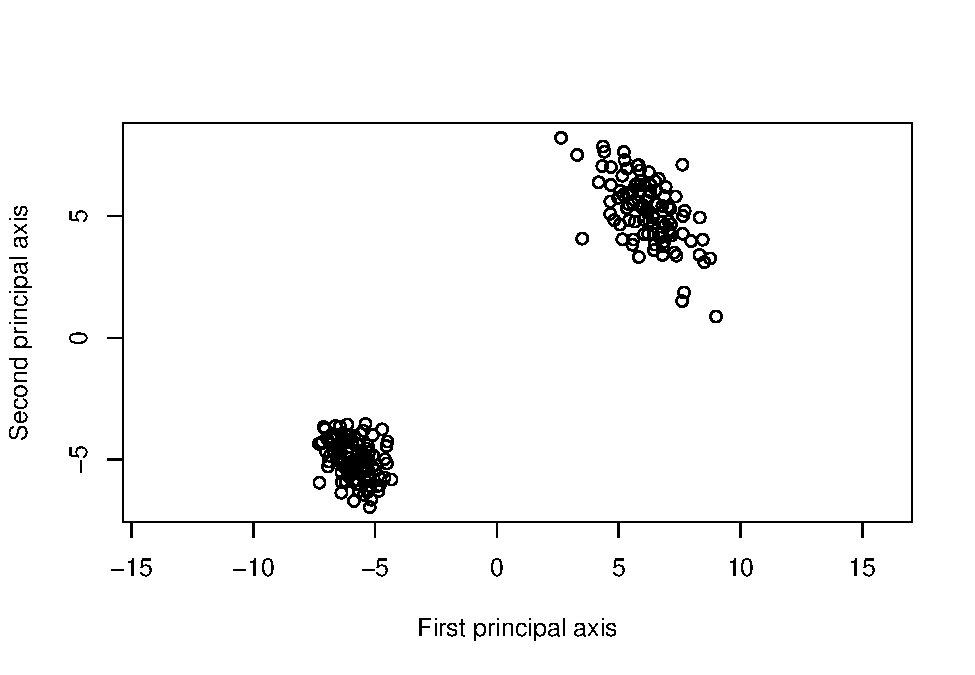
\includegraphics{P052020_Substructure_files/figure-latex/9th-2.pdf}

\begin{Shaded}
\begin{Highlighting}[]
\NormalTok{init <-}\StringTok{ }\KeywordTok{scale}\NormalTok{(}\KeywordTok{matrix}\NormalTok{(}\KeywordTok{runif}\NormalTok{(}\DecValTok{2}\OperatorTok{*}\NormalTok{n),}\DataTypeTok{ncol=}\DecValTok{2}\NormalTok{),}\DataTypeTok{scale=}\OtherTok{FALSE}\NormalTok{)}
\NormalTok{nmds.out <-}\StringTok{ }\KeywordTok{isoMDS}\NormalTok{(dists.all,}\DataTypeTok{k=}\DecValTok{2}\NormalTok{,}\DataTypeTok{y=}\NormalTok{init, }\DataTypeTok{trace =} \OtherTok{FALSE}\NormalTok{)}
\NormalTok{X =}\StringTok{ }\NormalTok{nmds.out}\OperatorTok{$}\NormalTok{points}
\KeywordTok{plot}\NormalTok{(X[,}\DecValTok{1}\NormalTok{],X[,}\DecValTok{2}\NormalTok{],}\DataTypeTok{asp=}\DecValTok{1}\NormalTok{,}\DataTypeTok{xlab=}\StringTok{"First principal axis"}\NormalTok{, }\DataTypeTok{ylab=}\StringTok{"Second principal axis"}\NormalTok{)}
\end{Highlighting}
\end{Shaded}

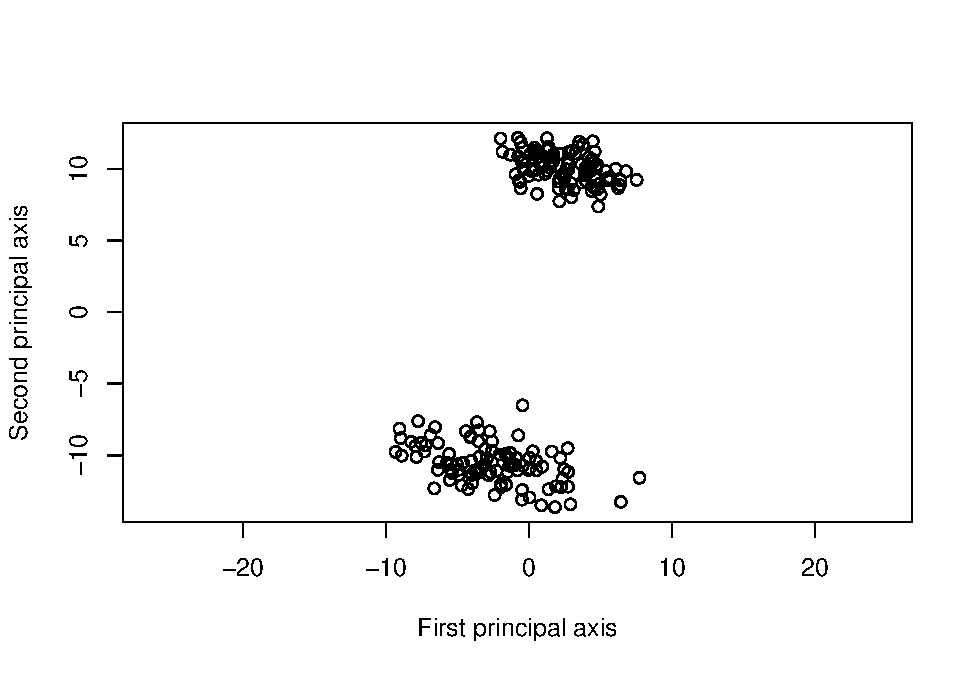
\includegraphics{P052020_Substructure_files/figure-latex/9th-3.pdf}

Initial configuration produces much much different results from the
results in the additional runs.

\begin{enumerate}
\def\labelenumi{\arabic{enumi}.}
\setcounter{enumi}{9}
\tightlist
\item
  (1p) Set the seed of the random number generator to 123. Then run
  isoMDS a hundred times, each time using a different random initial
  configuration using the instructions above. Save the final
  stress-value and the coordinates of each run. Report the stress of the
  best run, and plot the corresponding map.
\end{enumerate}

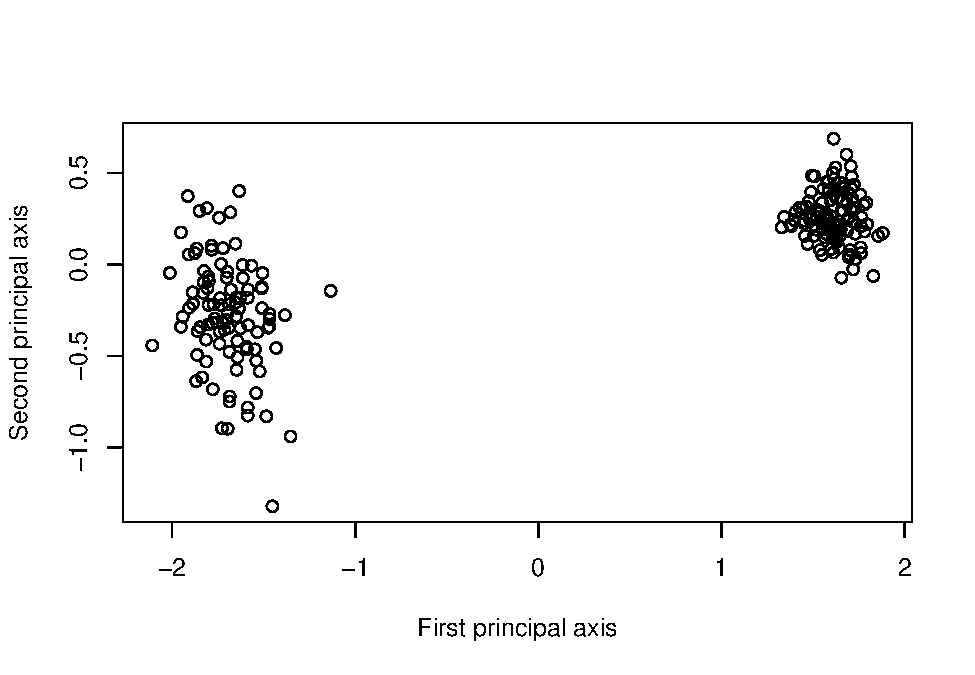
\includegraphics{P052020_Substructure_files/figure-latex/10th-1.pdf}

\begin{verbatim}
## [1] 11.40856
\end{verbatim}

The best stress value is 11.41, and the result of dimensionality
reduction is visible on the plot.

\begin{enumerate}
\def\labelenumi{\arabic{enumi}.}
\setcounter{enumi}{10}
\tightlist
\item
  (1p) Make again a plot of the estimated distances (according to your
  map of individuals of the best run) versus the observed distances, now
  for the two-dimensional solution of non-metric MDS. Regress estimated
  distances on observed distances and report the coefficient of
  determination of the regression.
\end{enumerate}

\begin{Shaded}
\begin{Highlighting}[]
\NormalTok{approx.dist =}\StringTok{ }\KeywordTok{as.matrix}\NormalTok{(}\KeywordTok{dist}\NormalTok{(X.best, }\DataTypeTok{method =} \StringTok{'manhattan'}\NormalTok{))}

\NormalTok{Dobs.vec <-}\StringTok{ }\NormalTok{dists.all[}\KeywordTok{lower.tri}\NormalTok{(dists.all)]}
\NormalTok{Dest.vec <-}\StringTok{ }\NormalTok{approx.dist[}\KeywordTok{lower.tri}\NormalTok{(approx.dist)]}

\KeywordTok{plot}\NormalTok{(Dobs.vec,Dest.vec,}\DataTypeTok{xlab=}\StringTok{"Observed"}\NormalTok{,}\DataTypeTok{ylab=}\StringTok{"Fitted"}\NormalTok{)}
\NormalTok{model =}\StringTok{ }\KeywordTok{lm}\NormalTok{(Dest.vec }\OperatorTok{~}\StringTok{ }\NormalTok{Dobs.vec)}
\KeywordTok{abline}\NormalTok{(model)}
\end{Highlighting}
\end{Shaded}

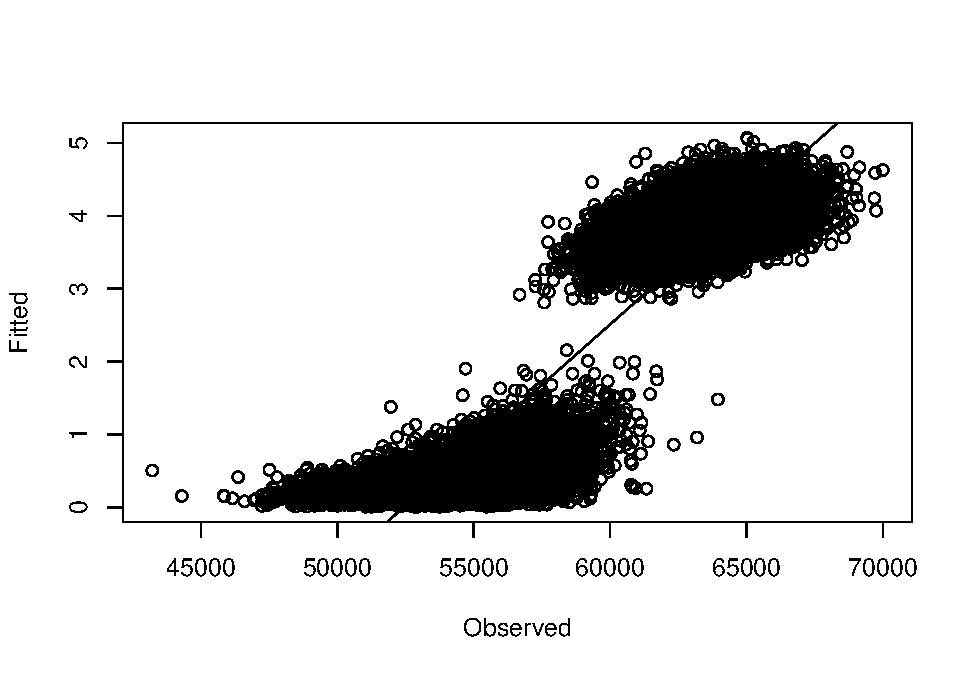
\includegraphics{P052020_Substructure_files/figure-latex/11th-1.pdf}

\begin{Shaded}
\begin{Highlighting}[]
\NormalTok{r2 =}\StringTok{ }\KeywordTok{summary}\NormalTok{(model)}\OperatorTok{$}\NormalTok{r.squared}
\NormalTok{r2}
\end{Highlighting}
\end{Shaded}

\begin{verbatim}
## [1] 0.8611736
\end{verbatim}

There are 2 ``groups'' which can be observed on the plot. Coefficient of
determination is 0.86.

\begin{enumerate}
\def\labelenumi{\arabic{enumi}.}
\setcounter{enumi}{11}
\tightlist
\item
  (1p) Compute the stress for a \(1, 2, 3, 4, \ldots, n\)-dimensional
  solution, always using the classical MDS solution as an initial
  configuration. How many dimensions are necessary to obtain a good
  representation with a stress below 5? Make a plot of the stress
  against the number of dimensions
\end{enumerate}

\begin{Shaded}
\begin{Highlighting}[]
\CommentTok{#stresses = c()}
\CommentTok{#for(k in 1:90) \{}
\CommentTok{#  nmds.out <- isoMDS(dists.all,k=k, trace = FALSE)}
\CommentTok{#  stresses = append(stresses, nmds.out$stress)}
\CommentTok{#\}}

\NormalTok{stresses =}\StringTok{ }\KeywordTok{read.csv}\NormalTok{(}\StringTok{'stresses.csv'}\NormalTok{)[,}\DecValTok{2}\NormalTok{]}

\KeywordTok{plot}\NormalTok{(}\DecValTok{1}\OperatorTok{:}\DecValTok{90}\NormalTok{, stresses, }\DataTypeTok{xlab =} \StringTok{'Number of dimensions'}\NormalTok{)}
\KeywordTok{abline}\NormalTok{(}\DecValTok{5}\NormalTok{,}\DecValTok{0}\NormalTok{)}
\end{Highlighting}
\end{Shaded}

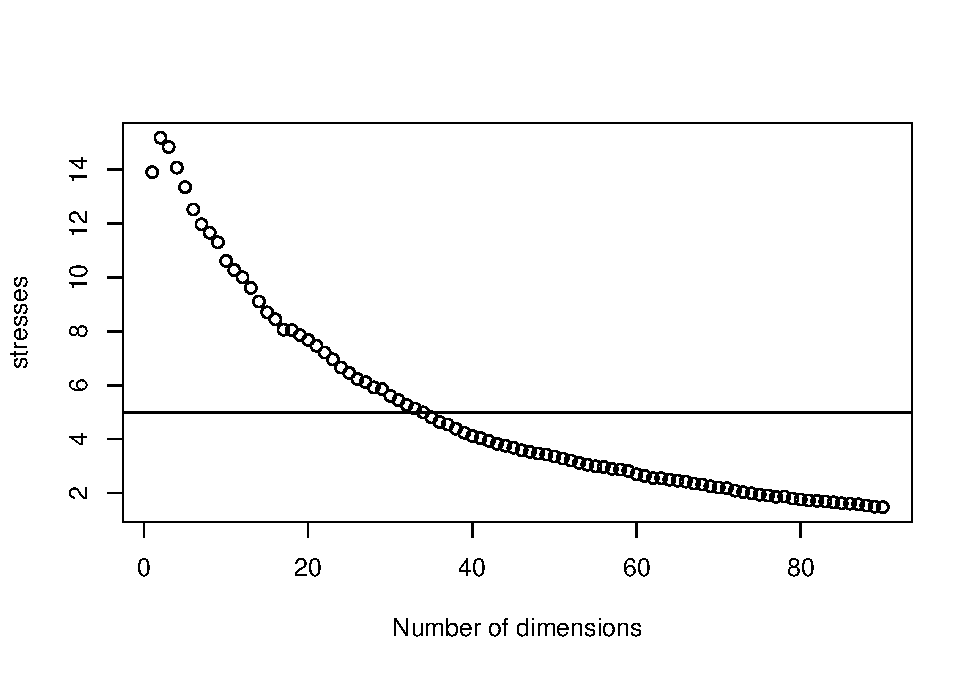
\includegraphics{P052020_Substructure_files/figure-latex/12th-1.pdf}

\begin{Shaded}
\begin{Highlighting}[]
\NormalTok{k.min =}\StringTok{ }\DecValTok{1}
\ControlFlowTok{for}\NormalTok{(i }\ControlFlowTok{in} \DecValTok{1}\OperatorTok{:}\KeywordTok{length}\NormalTok{(stresses)) \{}
  \ControlFlowTok{if}\NormalTok{(stresses[i] }\OperatorTok{<}\StringTok{ }\DecValTok{5}\NormalTok{) \{}
\NormalTok{    k.min =}\StringTok{ }\NormalTok{i}
    \ControlFlowTok{break}\NormalTok{;}
\NormalTok{  \}}
\NormalTok{\}}

\NormalTok{k.min}
\end{Highlighting}
\end{Shaded}

\begin{verbatim}
## [1] 34
\end{verbatim}

At least 34 dimensions are needed for stress to fall below 5. It is also
visible on the plot. We plotted only 90 values because the stress value
will only continue to reduce and it started to take a long time to
calculate the MDS for large \(n\).

\begin{enumerate}
\def\labelenumi{\arabic{enumi}.}
\setcounter{enumi}{12}
\tightlist
\item
  (2p) Compute the correlation matrix between the first two dimensions
  of a metric MDS and the two-dimensional solution of your best
  non-metric MDS. Make a scatterplot matrix of the 4 variables. Comment
  on your findings.
\end{enumerate}

\begin{Shaded}
\begin{Highlighting}[]
\NormalTok{X.non.metric =}\StringTok{ }\NormalTok{X.best }
\KeywordTok{cor}\NormalTok{(X.mds, X.non.metric)}
\end{Highlighting}
\end{Shaded}

\begin{verbatim}
##            [,1]        [,2]
## [1,] 0.99736763  0.75047759
## [2,] 0.01153539 -0.05454761
\end{verbatim}

\begin{Shaded}
\begin{Highlighting}[]
\KeywordTok{plot}\NormalTok{(X.mds[,}\DecValTok{1}\NormalTok{], X.non.metric[,}\DecValTok{1}\NormalTok{])}
\end{Highlighting}
\end{Shaded}

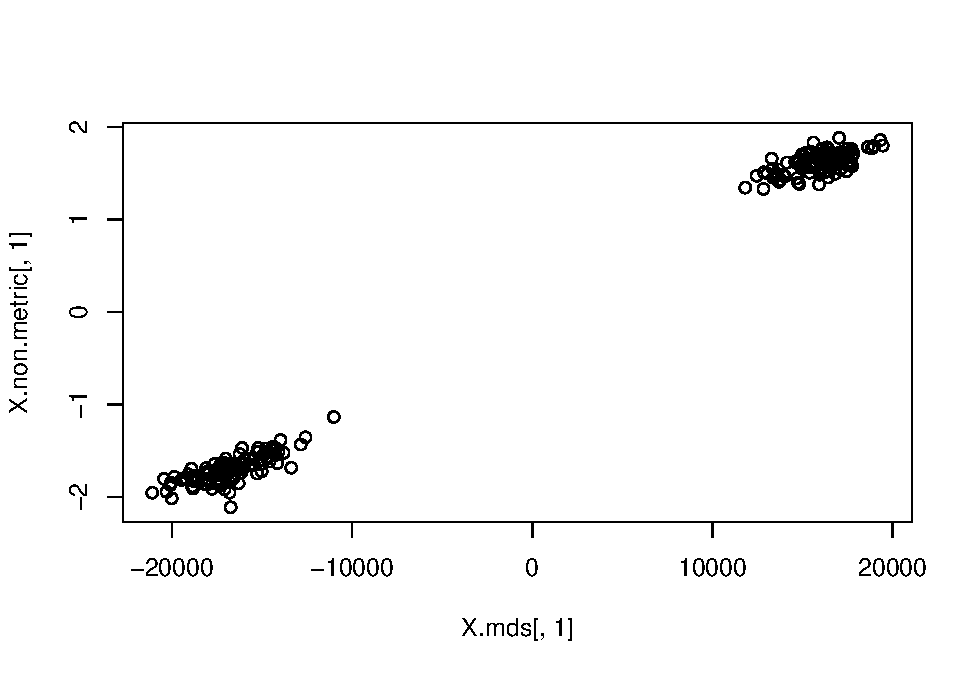
\includegraphics{P052020_Substructure_files/figure-latex/13th-1.pdf}

\begin{Shaded}
\begin{Highlighting}[]
\KeywordTok{plot}\NormalTok{(X.mds[,}\DecValTok{1}\NormalTok{], X.non.metric[,}\DecValTok{2}\NormalTok{])}
\end{Highlighting}
\end{Shaded}

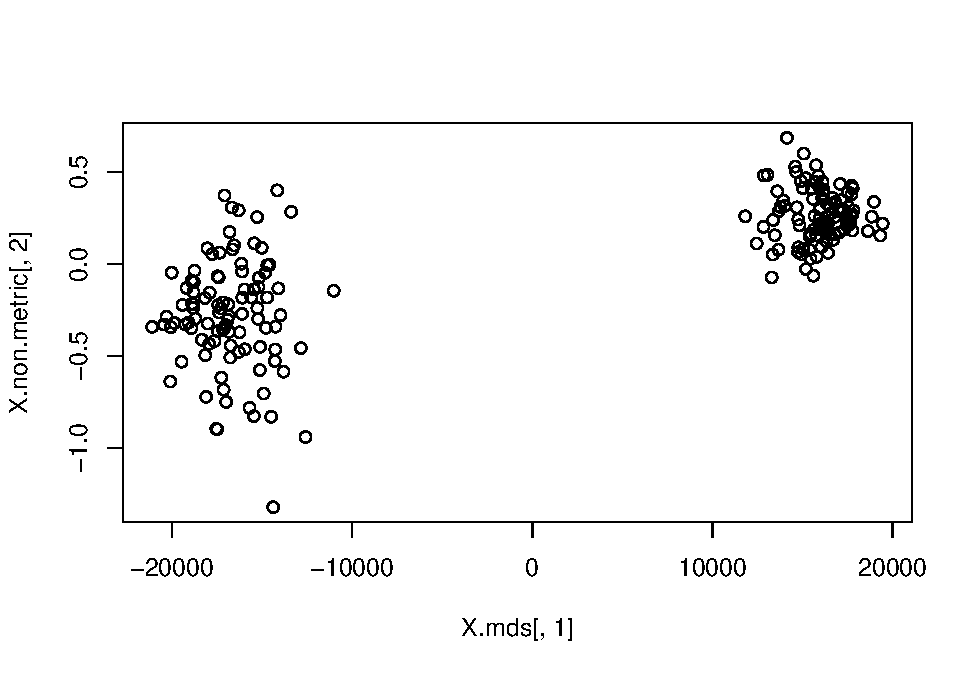
\includegraphics{P052020_Substructure_files/figure-latex/13th-2.pdf}

\begin{Shaded}
\begin{Highlighting}[]
\KeywordTok{plot}\NormalTok{(X.mds[,}\DecValTok{2}\NormalTok{], X.non.metric[,}\DecValTok{1}\NormalTok{])}
\end{Highlighting}
\end{Shaded}

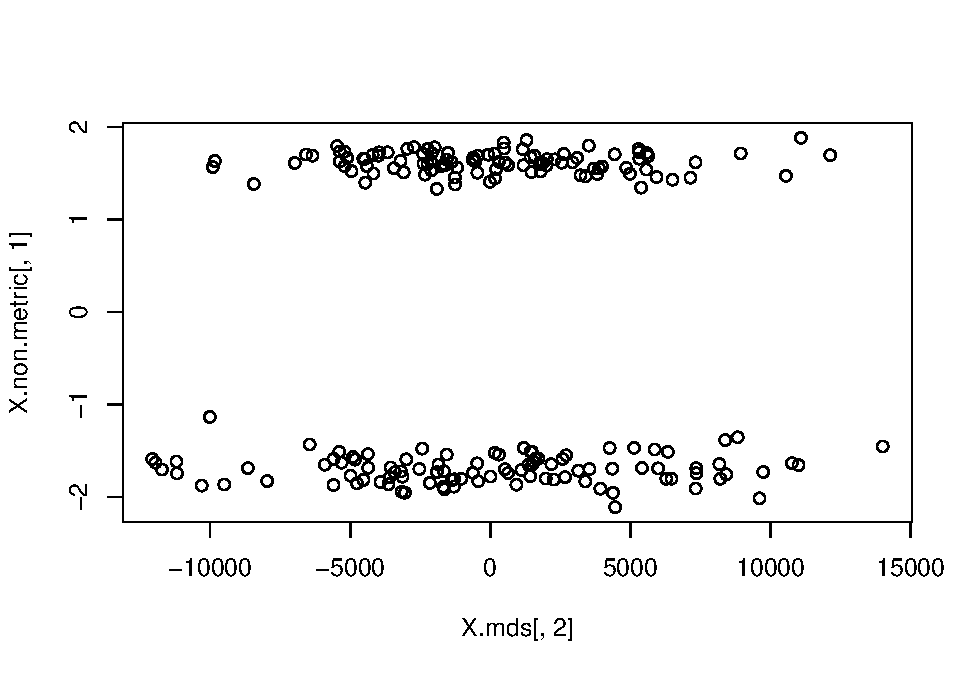
\includegraphics{P052020_Substructure_files/figure-latex/13th-3.pdf}

\begin{Shaded}
\begin{Highlighting}[]
\KeywordTok{plot}\NormalTok{(X.mds[,}\DecValTok{2}\NormalTok{], X.non.metric[,}\DecValTok{2}\NormalTok{])}
\end{Highlighting}
\end{Shaded}

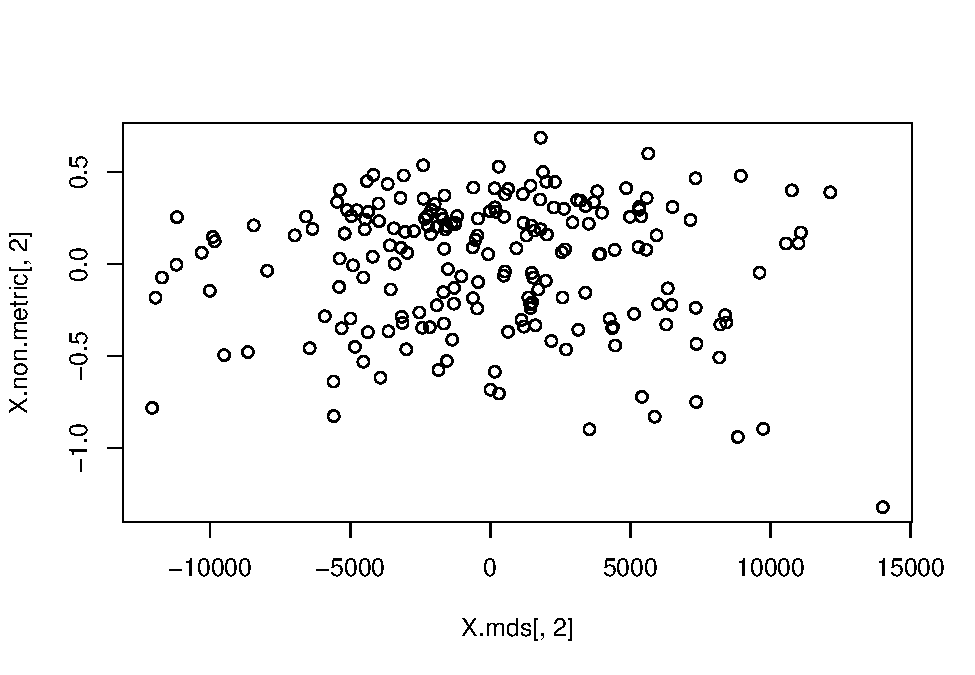
\includegraphics{P052020_Substructure_files/figure-latex/13th-4.pdf} The
first dimensions of both matrices (1,1) are highly positively correlated
(1st plot) and second dimensions of both matrices (2,2) are completely
uncorrelated (4th plot). In other case of (1,2) we can observe a
correlation of roughly 0.75 which is a pretty high positive correlation
and that is also observable on the plot, since there is some kind of
straight line which could be drawn. In the case (2,1) we observe that
for each value of metric coordinate there are roughly 2 possible levels
which can be achieved (-2 and 2), but there is no correlation between
the 2 dimensions.

\end{document}
